\documentclass{article} % this tells LaTeX to make an article (as opposed to a book, for example)

\usepackage[utf8]{inputenc}
\usepackage[english]{babel}
\usepackage{indentfirst}


\usepackage{amsmath, % this adds functions for formatting equations nicely
      amssymb,
      multirow,
      multicol,
      amsthm,
      todonotes, % add to do notes with \todo command
      mathtools,
      stmaryrd,
      tikz } % this gives us lots of greek symbols
\usepackage{titling}
\usepackage{pgfplots}
\usepackage[round]{natbib} % extra functionality for citations
 

\newcommand*\circled[1]{\tikz[baseline=(char.base)]{
            \node[shape=circle,draw,inner sep=2pt] (char) {#1};}}
\newcommand*\circleditem{%
   \stepcounter{enumi}\item[\circled{\theenumi}]}



\setlength{\parskip}{1em}

\newtheorem{theorem}{Theorem} 
\newtheorem{definition}{Definition} % this lets us create definition blocks as below
\newtheorem{remark}{Remark}


\title{A Graph Theoretical Approach to Revealed Preferences and Efficiency Indices}
\author{...}
\begin{document}

\maketitle

\begin{abstract}
Prior literature on consumer behavior and revealed preferences focus on the necessary requirements of choice data to satisfy consistency but often neglect developing algorithms to test for those requirements for large datasets. Additionally, existing efficiency indices proposed by \citet{Afriat1967The-Construction-of-Utility-Functions-from-Expenditure-Data} and \citet{Varian1990Goodness-of-fit-in-optimizing-models} requires exhausting computations. This paper proposes new algorithms to test for consumer maximization and calculate efficiency indices through a graph theoretical approach. The paper will place existing theory in a graph theoretical context and develop a new method to directly calculate efficiency indices.
\end{abstract}

\section*{Revealed Preferences as a Directed Graph}

Suppose an individual is observed over $k$ (a finite number of) periods. Let $\mathcal{X}=\{X_1,\ldots,X_k\}$ be the set of quantity vectors such that $\forall i\in\{1,\ldots,k\}$, $X_i=(x_{i1},\ldots,x_{in})$, where $x_{ij}$ represents the number of good $j$ bought at time $i$. Further, let $\mathcal{P}=\{P_1,\ldots,P_k\}$ be the set of price vectors constructed in similar fashion as the quantity vectors. We then define a following set of relations between elements of $\mathcal{X}$:

\begin{definition} \leavevmode
\begin{enumerate}
  \circleditem For $X_i, X_j\in\mathcal{X}$, we say $X_i$ is \textbf{directly revealed preferred} to $X_j$ if $P_iX_i\geq P_iX_j$. We will denote this as $X_i R_D X_j$.
  \circleditem For $X_i, X_j\in\mathcal{X}$, we say $X_i$ is \textbf{strictly directly revealed preferred} to $X_j$ if $P_iX_i>P_iX_j$. We will denote this as $X_i R_{SD} X_j$.
  \circleditem For $X_i, X_j\in\mathcal{X}$, we say $X_i$ is \textbf{revealed preferred} to $X_j$ if there exists some sequence $\{X^m\}_{m=1}^{M}$ such that, $\forall m\in\{1,\ldots,M\}$, the following holds:
  \begin{itemize} 
    \item $X^m\in\mathcal{X}$
    \item $X_i R_D X^1$
    \item $X^m R_D X^{m+1}$
    \item $X^M R_D X_j$
  \end{itemize} 
  We will denote this as $X_i R X_j$.
\end{enumerate}
\end{definition}
This definition comes directly from \citet{Varian1982The-Nonparametric-Approach-to-Demand-Analysis}. Note that \circled{1} and \circled{2} simply state that $X_i$ is (strictly) directly revealed preferred to $X_j$ if $X_j$ (costs less) is available at the prices when $X_i$ was chosen. For \circled{3}, we see that $R$ is the transitive closure on $R_D$, as $X_iRX_j$ if there is some sequence $X$'s that ``connects'' $X_i$ to $X_j$ through a chain of directly revealed preferences. Using these relations, we define the following set of axioms, as shown in \citet{Varian1982The-Nonparametric-Approach-to-Demand-Analysis} and \citet{BanerjeeMurphy2015A-Caveat-for-the-Application-of-the-Critical-Cost-Efficiency-Index-in-induced-budget-experiments}:

\begin{definition} \leavevmode
\begin{enumerate}
  \circleditem A set of choice data satisfies the \textbf{Weak Axiom of Revealed Preferences (WARP)} if for all bundles $X_i$ and $X_j$ in $\mathcal{X}$, if $X_i$ is directly revealed preferred to $X_j$, then $X_j$ is not directly revealed preferred to $X_i$.
  \circleditem A set of choice data satisfies the \textbf{Strong Axiom of Revealed Preferences (SARP)} if for all bundles $X_i$ and $X_j$, if $X_i$ is revealed preferred to $X_j$, then $X_j$ is not revealed preferred to $X_i$.
  \circleditem A set of choice data satisfies the \textbf{Generalized Axiom of Revealed Preferences (GARP)} if for all bundles $X_i$ and $X_j$, if $X_i$ is revealed preferred to $X_j$, then $X_j$ is not strictly directly revealed preferred to $X_i$.
  \circleditem A set of choice data satisfies the \textbf{Weak Generalized Axiom of Revealed Preferences (WGARP)} if for all bundles $X_i$ and $X_j$, if $X_i$ is directly revealed preferred to $X_j$, then $X_j$ is not strictly directly revealed preferred to $X_i$.
\end{enumerate}
\end{definition}

\begin{remark}
The SARP requirement can also be written as: ``A set of choice data satisfies the \textbf{Strong Axiom of Revealed Preferences (SARP)} if for all bundles $X_i$ and $X_j$, if $X_i$ is revealed preferred to $X_j$, then $X_j$ is not \emph{directly} revealed preferred to $X_i$.''. This equality is shown in \citet{Varian1982The-Nonparametric-Approach-to-Demand-Analysis} and can be easily seen in a graph theoretical approach to the axiom.
\end{remark}

\begin{remark}
If a consumer exhibits maximizing behavior, then their set of choice data will satisfy WARP. However, the converse isn't necessarily true when X and Y represent bundles from commodity spaces higher than two dimensions (i.e. there are more than two available goods and thus, $X$, $Y$, and $P$ are n-dimensional vectors such that $n> 2$)  See \citet{Rose1958Consistency-of-Preference:-The-Two-Commodity-Case}.
\end{remark}

\begin{remark}
\label{rmk:Remark 3}
The key difference between SARP and GARP requirements are that GARP allows consumers to have multiple bundles that maximizes utility under the same price levels (i.e. consumers are allowed to exhibit preferences that treat goods as perfect substitutes of each other).
\end{remark}
Consider the following example for Remark \ref{rmk:Remark 3}. Let good $i$ and good $j$ be perfect 1-to-1 substitutes for an individual. Additionally, let $p_i=\alpha$, $p_j=\alpha$ at time $t$ and $p_i=\beta$, $p_j=\beta$ at time $t+1$. One can see that, given the underlying preference of the individual and the price ratios, the bundle selected by the consumer is completely random. Suppose the individual purchases 1 unit of good $i$ at time $t$ with no purchases of good $j$ and chooses 1 unit of good $j$ at time $t+1$ with no purchases of good $i$. Although this behavior is completely rational for the individual given their underlying preference (perfect substitutes), a set of choice data exhibit such behavior would fail WARP and SARP as $X_{t} R_D X_{t+1}$ but $X_{t+1} R_D X_{t}$. This is because $P_tX_t=\alpha\geq\alpha=P_tX_{t+1}$ and $P_{t+1}X_{t+1}=\beta\geq\beta=P_{t+1}X_t$. However, it's clear that this set of choice data will pass WGARP and GARP. The example can be illustrated with the following diagram:
\begin{center}
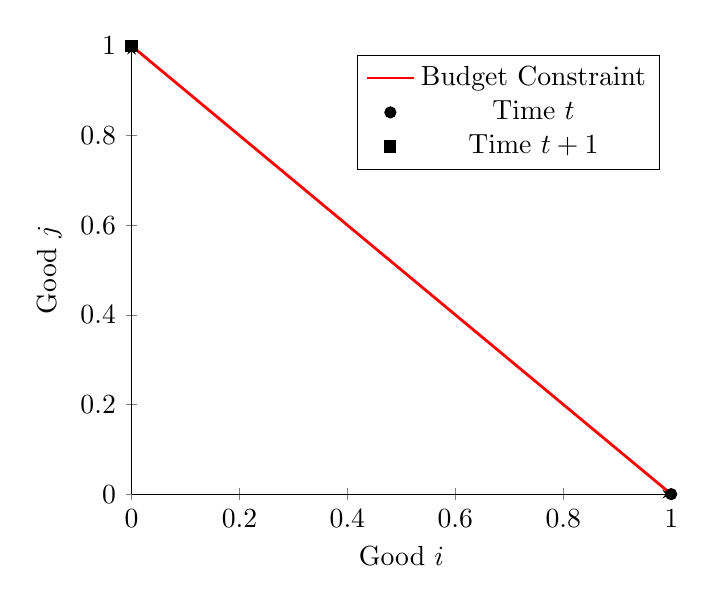
\begin{tikzpicture}
    \begin{axis}[
    axis lines = left,
    xlabel = Good $i$,
    ylabel = Good $j$
]
  \addplot [
    domain=0:1, 
    samples=2, 
    color=red,
    line width=1pt
]
{1-x};
\addlegendentry{Budget Constraint}
\addplot [only marks] table {
1 0
};
\addlegendentry{Time $t$}
\addplot [only marks, mark=square*] table {
0 1
};
\addlegendentry{Time $t+1$}
    \end{axis}
\end{tikzpicture}
\end{center}
\noindent
Note the red line represent both the indifference curves \emph{and} budget constraints at time $t$ both times. Under these conditions, any choice along the budget constraint is rational. 

The following table summarizes the requirements for each of the axioms:

\renewcommand{\arraystretch}{1.5}
\begin{center}
\begin{tabular}{ c|c|c } 
Axiom & If $\ldots$ & Then $\ldots$ \\\hline
WARP&$X_i \mathbf{R_D} X_j$&$\neg(X_j \mathbf{R_D} X_i)$ \\
SARP&$X_i \mathbf{R} X_j$&$\neg(X_j \mathbf{R} X_i)$ \\
WGARP&$X_i  \mathbf{R_D} X_j$&$\neg(X_j \mathbf{R_{SD}} X_i)$ \\
GARP&$X_i \mathbf{R} X_j$&$\neg(X_j  \mathbf{R_{SD}} X_i)$
\end{tabular}
\end{center}
\renewcommand{\arraystretch}{1}



\bibliographystyle{plainnat}
\bibliography{bibliography}

\end{document}
